\documentclass[11pt]{article} % scrbook otro formato
\usepackage[utf8]{inputenc}
\usepackage[spanish,es-tabla,es-nodecimaldot]{babel}

% Paquetes

\usepackage{amsmath}
\usepackage{amsthm}
\usepackage{amsfonts}
\usepackage{amssymb}
\usepackage{makeidx}
\usepackage{graphicx}
\usepackage{lmodern}
%\usepackage{kpfonts}
\usepackage{fancyhdr}
\usepackage{geometry}
\usepackage{lastpage}
\usepackage{array} % Para fjar tamaño de columnas
\RequirePackage{siunitx}
\usepackage{extramarks} % Para poder usar firstleftmarks
\usepackage[version=4]{mhchem} % Para poder usar formulas de reacciones nucleares
\usepackage{xcolor}
%\usepackage{newtxtext, newtxmath} % Cambia la fuente (pero mola)
\usepackage{tcolorbox}

\newtcolorbox{mybox}{colback=black!5!white,
	colframe=black!75!black}

%##############################################################################
%######### Ponemos el decimal con . ###########################################
%##############################################################################

\sisetup{output-decimal-marker={.},
	% exponentes ------------------------
	%exponent-mode=threshold,
	%exponent-thresholds=-3:2, % non usar exponentes 10^{-2,-1, 0, 1}
	% redondear -------------------------
	% round-mode=figures, % cifras sig
	% round-mode=places, % cantos decimales
	round-mode=uncertainty, % cifras sig da incerteza (necesario usar erro)
	round-precision=2,
	uncertainty-mode = separate,
	print-unity-mantissa=false,
	% unidades --------------------------
	inter-unit-product = \ensuremath{{}\cdot{}}, % separacion entre unidades
	% per-mode=power-positive-first, % so furrula con metodo interpretado puro
	inline-per-mode=single-symbol,
	display-per-mode=fraction,
}

%##############################################################################
%######### Para codigo python #################################################
%##############################################################################

\definecolor{codegreen}{rgb}{0,0.6,0}
\definecolor{codegray}{rgb}{0.5,0.5,0.5}
\definecolor{codepurple}{rgb}{0.58,0,0.82}
\definecolor{backcolour}{rgb}{0.95,0.95,0.92}

\usepackage{listings}


%\lstdefinestyle{mystyle}{	backgroundcolor=\color{backcolour},   	commentstyle=\color{codegreen},	keywordstyle=\color{magenta},	numberstyle=\tiny\color{codegray},	stringstyle=\color{codepurple},	basicstyle=\ttfamily\footnotesize,	breakatwhitespace=false,         	breaklines=true,                 	captionpos=b,                    	keepspaces=true,                 	numbers=left,                    	numbersep=5pt,                  	showspaces=false,                	showstringspaces=false,	showtabs=false,                  	tabsize=2}

%\lstset{style=mystyle}
%\usepackage{background}     % Para manejar el fondo


%##############################################################################
%######### Tipo de fuente #################################################
%##############################################################################

%\usepackage{kpfonts}

%\usepackage{helvet} 
%\renewcommand{\familydefault}{\sfdefault}.

%\usepackage{fontspec} % Paquete necesario para seleccionar fuentes
%\setmainfont{Verdana} % Cambia la fuente principal a Verdana


%##############################################################################
%######### Geometría #################################################
%##############################################################################

\geometry{a4paper, total={152mm,237mm}, left=31mm, top=30mm}



%##############################################################################
%######### Formatos capítulo #################################################
%##############################################################################

%\usepackage[lmodern]{quotchap}
%\usepackage[Bjornstrup]{fncychap}

% Para el Bjornstrup
%\ChNumVar{\fontsize{76}{80}\usefont{OT1}{pzc}{m}{n}\selectfont}
%\ChTitleVar{\raggedright\Huge\sffamily\bfseries}


%##############################################################################
%######### Hiperreferenias #################################################
%##############################################################################


\usepackage[colorlinks=true,allcolors=blue]{hyperref} % Crea las


%##############################################################################
%######### Formato de pagina #################################################
%##############################################################################

%\renewcommand{\chaptermark}[1]{\markboth{\chaptername\ \thechapter.\ #1}{}}
\renewcommand{\sectionmark}[1]{\markright{\thesection.\ #1}}

\setlength{\headsep}{27pt} % Distancia entre la cabezera y el texto
\setlength{\footskip}{30pt} % Distancia entre el pie de pagina y el texto
\pagestyle{fancy}
\fancyhf{}
\fancyhead[LE]{\rightmark} % L,R,C-> left, right, center [LE,RO]
\fancyhead[RO]{\rightmark} % E,O -> even (par), odd (impar)
\fancyhead[LO,RE]{Daniel Vázquez Lago}
\fancyfoot[CE,CO]{\thepage}
\renewcommand{\headrulewidth}{1pt} % Cambiamos el grosor de la linea de arriba
\renewcommand{\footrulewidth}{0pt}



%##############################################################################
%#########  Modificar caption #################################################
%##############################################################################

\usepackage[font=small, justification=centering]{caption}  % Configura las captions



%##############################################################################
%######### Comandos propios #################################################
%##############################################################################

\newcommand{\parentesis}[1]{\left( #1  \right)} 
\newcommand{\parciales}[2]{\frac{\partial #1}{\partial #2}}
\newcommand{\pparciales}[2]{\parentesis{\parciales{#1}{#2}}}
\newcommand{\ccorchetes}[1]{\left[ #1  \right]}
\newcommand{\D}{\mathrm{d}}
\newcommand{\derivadas}[2]{\frac{\D #1}{\D #2}}

\newcommand{\tquad}{\quad \quad \quad}
\newcommand{\vnabla}{\vec{\nabla}}

\newcommand{\Ocal}{\mathcal{O}}
\newcommand{\Ncal}{\mathcal{N}}
\newcommand{\Hcal}{\mathcal{H}}

\newcommand{\logd}{\log_{10}}

\newcommand{\eV}{\text{eV}}
\newcommand{\cm}{\text{cm}}
\newcommand{\cmm}{\text{cm}^{-1}}
\newcommand{\fm}{\text{fm}}
\newcommand{\He}{\text{He}}
\newcommand{\p}{\text{p}}
\newcommand{\e}{\text{e}}
\newcommand{\cte}{\text{cte}}


% Comandos vectoriales

\newcommand{\an}{\mathbf{a}}
\newcommand{\bn}{\mathbf{b}}
\newcommand{\dn}{\mathbf{d}}
\newcommand{\jn}{\mathbf{j}}
\newcommand{\lnn}{\boldsymbol{\ell}}
\newcommand{\lnnn}{\boldsymbol{l}}
\newcommand{\kn}{\mathbf{k}}
\newcommand{\pn}{\mathbf{p}}
\newcommand{\qn}{\mathbf{q}}
\newcommand{\rn}{\mathbf{r}}
\newcommand{\sn}{\mathbf{s}}
\newcommand{\un}{\mathbf{u}}
\newcommand{\vn}{\mathbf{v}}
\newcommand{\xn}{\mathbf{x}}
\newcommand{\yn}{\mathbf{y}}
\newcommand{\qndot}{\dot{\qn}}

\newcommand{\unovec}{\vec{\mathbf{1}}}

\newcommand{\alphan}{\boldsymbol{\alpha}}
\newcommand{\sigman}{\boldsymbol{\sigma}}
\newcommand{\pin}{\boldsymbol{\pi}}


\newcommand{\An}{\mathbf{A}}
\newcommand{\Bn}{\mathbf{B}}
\newcommand{\En}{\mathbf{E}}
\newcommand{\Gn}{\mathbf{G}}
\newcommand{\Jn}{\mathbf{J}}
\newcommand{\Kn}{\mathbf{K}}
\newcommand{\Ln}{\mathbf{L}}
\newcommand{\Rn}{\mathbf{R}}
\newcommand{\Sn}{\mathbf{S}}
\newcommand{\Tn}{\mathbf{T}}
\newcommand{\In}{\mathbf{I}}

\newcommand{\hnn}{\hat{\mathbf{n}}}
\newcommand{\hnr}{\hat{\mathbf{r}}}
\newcommand{\hnz}{\hat{\mathbf{z}}}
\newcommand{\hnx}{\hat{\mathbf{x}}}
\newcommand{\hny}{\hat{\mathbf{y}}}
\newcommand{\hnu}{\hat{\mathbf{u}}}
\newcommand{\hnR}{\hat{\mathbf{R}}}
\newcommand{\hnv}{\hat{\mathbf{v}}}
\newcommand{\hnk}{\hat{\mathbf{k}}}
\newcommand{\hni}{\hat{\mathbf{i}}}
\newcommand{\hnj}{\hat{\mathbf{j}}}
\renewcommand{\hnk}{\hat{\mathbf{k}}}





%##############################################################################
%######### Teoremas/definiciones #################################################
%##############################################################################

%\theoremstyle{definition}
%\newtheorem{definition}{Definición}[chapter]
%\theoremstyle{theorem}
%\newtheorem{theorem}{Teorema}[chapter]




%##############################################################################
%######### Referncia para euccaiones y figuras ################################
%##############################################################################

%\numberwithin{equation}{section}
%\numberwithin{figure}{section}




%##############################################################################
%######### Documento #################################################
%##############################################################################


\author{Daniel Vazquez Lago}
\title{Simulación en física de materiales}


\begin{document}	
	
\maketitle
\newpage
\tableofcontents
\section{Objetivos}

El objetivo de esta segunda entrega de la asignatura es llegar a la posición de equilibrio de un sistema de 500 partículas, con una densidad $\rho=0.5$ y una energía $E=575$ (variables reducidas) a partir de una posición inicial fcc. Sin embargo para llegar al equilibrio primero debemos avanzar en el tiempo, es decir, hacer una simulación. En este proyecto veremos qué debemos implementar para poder calcular posiciones temporales sucesivas hasta la posición deseada. En el optativo 1 dos veremos si, realmente con los pasos logrados en este ejercicio se llega o no al equilibrio.

\section{Organización} \label{Sec:02}

En esta sección mencionare como están organizados el proyecto. En primer lugar hay que decir que, por motivos de organización personal, he creado una carpeta llamada \textit{Datos} donde se almacenan todos los \texttt{.dat} de todos los proyectos. Sin embargo para que se guarden correctamente he supuesto que se ejecuta desde el proyecto, esto es, desde el \texttt{.exe} que se genera al construir el proyecto. De hacerlo de otro modo esto llevaría a un error. En segundo lugar, se puede ver que tal y como recomendó el profesor, hay una carpeta donde guardo todos los archivos \texttt{.f95} (llamada \textit{Programas fuente}) y otra donde esta el proyecto \texttt{.ftn95p}, para así poder reusarlos y que esté bien ordenado. Una breve descripción de los archivos:

\begin{itemize}
	\item \textbf{Mod\_01\_Def\_prec}: modulo usado para definir las precisiones doble precisión y entero, permitiéndo usar datos con más cifras decimales.
	\item \textbf{Mod\_02\_Variables\_comunes}: nos permite pasar las variables comunes entre las diferentes subrutinas y programas sin necesidad de definirlos en los propios programas.
	\item \textbf{Mod\_03\_Interface}: módulo que nos permite detectar errores a la hora de introducir datos en las subrutinas, así como detectarlos en las variables de salida de las mismas.
	\item \textbf{Sub\_Potlj:} subrutina en la cual introducimos las posiciones y el número de partículas como variables de entrada y nos devuelve las aceleraciones/fuerzas, así como la energía potencial del sistema y sus derivadas respecto al volumen (primera y segunda).
	\item \textbf{Sub\_Verlet:} subrutina la cual recibe una configuración inicial en el instante $t$ y devuelve la nueva configuración inicial en $t+\Delta t$ (para esto esta subrutina llama a \texttt{Sub\_Potlj}). Además también obtenemos con ella la energía potencial.
	\item \textbf{Pro\_Equilibracion:} programa principal. Su principal función es leer la configuración inicial (partiendo de la fcc o bien de alguna más estable, siempre que verifique $E=-575$), y mediante un lazo iterar el número de veces que se desee la subrtuina \texttt{Sub\_Verlet}, avanzando un tiempo total $k\Delta t$, donde $k$ es el número de pasos y $\Delta t$ el intervalo temporal entre cada uno. Además escribirá en el mismo archivo que se leyó la configuración final, así como en nuevos archivos de datos las energías cinética, potencial y total; así como las velocidades (entre otros datos), en pos de ver si realmente se ha equilibrado.
\end{itemize}


\section{Simulación}

En esta sección vamos a ver como se hace la simulación, esto es, como calculamos la posición, velocidad... en la configuración $t+\Delta t$ a partir de los datos en $t$ (o anteriores, esto es, $t  - \Delta t, \ t - 2 \Delta t$). En realidad, obtener la posición temporal siguiente no es otra cosa que resolver una ecuación diferencial (ecuaciones del movimiento de las partículas) a través de metodos diferenciales finitos, que son los únicos con los que puede trabajar el ordenador. Estos métodos diferenciales finitos nos llevarán a dos errores diferentes que tendremos que minimizar todo lo que podamos con el propósito de obtener la simulación mas acertada con el modelo del que disponemos. 

De esta manera en la primera parte de la sección discutiremos desde un punto de vista completamente teórico qué método vamos a usar y como vamos a minimizar el error, mientras que en la segunda parte vamos a explicar brevemente como lo implementamos en fortran.

\subsection{Introducción teórica}

Para conocer la posición de las partículas en el instante de $t + \Delta t$, si $\Delta t$ es suficientemente pequeña, podemos desarrollar la serie de Taylor de $\rn(t+\Delta t)$

\begin{eqnarray}
	\rn(t+\Delta t) = \rn (t) + \dot{\rn} (t) \Delta t + \frac{1}{2} \ddot{\rn} (t) (\Delta T)^2 + \frac{1}{6} \dddot{\rn} (t) (\Delta T)^3 + \ldots \label{Ec:01}
\end{eqnarray}
Conocidos los valores de $\rn,\dot{\rn}$, $\ddot{\rn}...$ podremos calcular la nueva posición. Sin embargo esto nos lleva a dos preguntas ¿A qué nos referimos con $\Delta t$ suficientemente pequeña?¿Qué valor le asignamos a las variables $\dot{\rn}...$? La primera pregunta la responderemos en el apartado \ref{Subsec:03-01} mientras que la segunda en el apartado \ref{Subsec:03-02}. 


\subsubsection{Minimización del error y estabilidad} \label{Subsec:03-01}

Existen dos tipos de errores asociados a los algoritmos de metodos diferenciales finitos: el error de trucación global (egt) y el error de redondeo global (ert).

\begin{itemize}
 \item El error de truncación viene determinado por el método que usemos para resolver la ecuación diferencial. En general el orden del error de truncación viene depende del orden en el que cortemos el desarrollo de Taylor (\ref{Ec:01}). Nosotros tendremos en cuenta hasta $(\Delta T)^2$, por lo que el error de truncamiento será generado por los términos de orden 3 o superior. Cuanto más grande sea $\Delta t$, más grande será el error de truncamiento. De hecho, si $\Delta t>1$, tendremos que el error de truncamiento será infinito. Por eso mismo es obligatorio que se verifica que $\Delta t<1$. Cuan más bajo sea $\Delta t$ este error será mucho menor. Otra manera de minimizar este error sería coger términos de orden superior, tal y como se hace en el algoritmo Gear. 

 \item El error redondeo depende en última instancia de las cifras tenidas en cuenta a la hora de trabajar el ordenador. Este error se hace más grande a medida que $\Delta t$ disminuye, ya que llega un momento en el que el error por trabajar con números finitos se hace cada vez más significativo en $\Delta t$.  
\end{itemize}

Otra elemento que afecta a las simulaciones es la estabilidad. Además de tratar de reducir el error, es importante ver como el algoritmo propaga los diferentes errores. Si el error que se propaga con cada interacción es cada vez mayor, diremos que el algoritmo es inestable. Por otro lado, si los errores no aumentan, cancelándose mutuamente, diremos que el método es estable. Dado que muchas veces la dinámica molecular trata con ecuaciones diferenciales no ordinarias, hacer una análisis soobre la estabilidad analíticamente puede ser complicado. La mejor manera de conocer el $\Delta t$ crítico (aquel a partir del cual el sistema es inestable) es hacer diferentes pruebas. 

Consecuentemente ni podemos tomar un $\Delta t$ muy grande, ni tampoco un $\Delta t$ ridículamente pequeño. La única manera de saber cual es el mejor $\Delta t$ será haciendo diferentes pruebas (tanto para la estabilidad como para el error global), y ver cual funciona mejor. Nosotros usaremos $\Delta t = 0.0001$, que, como veremos, funciona bastante bien.  \\



\subsubsection{Algoritmo velocity Verlet} \label{Subsec:03-02}

Para conocer los valores de los diferentes $\dot{\rn}$ debemos usar las ecuaciones canónicas de nuestro hamiltoniano $\Hcal$ (aunque en PVE el resultado sea trivial, puede que no lo sea en otras colectividades), dado por la energía cinética y un potencial que solo depende de la posición:

\begin{equation}
	\Hcal = \sum_{i=1} \frac{\pn_i^2}{2m} + \varphi (\rn_i)
\end{equation}
donde $\varphi(\rn_i)$ viene dado por el \textit{potencial Lennard-Jones}. Si definimos la velocidad como $\pn=m\vn$ y la aceleración como $\ddot{\rn}_i = \an_i$, tenemos que:

\begin{equation}
	\dot{\rn}_i = \parciales{\Hcal}{\pn_i} = \frac{\pn_i}{m} = \vn_i
\end{equation}

\begin{equation}
	\dot{\pn}_i = - \parciales{\Hcal}{\rn_i} \Rightarrow  m \ddot{\rn}_i = - \parciales{\varphi(\rn_i)}{\rn_i} \Rightarrow \an_i =  - \frac{1}{m} \parciales{\varphi(\rn_i)}{\rn_i}
\end{equation}
Reescribimos (\ref{Ec:01}) como
\begin{equation}
	\rn(t+\Delta t) = \rn(t) + \vn(t) \Delta t + \frac{1}{2} \an (t) (\Delta T)^2
\end{equation}
donde hemos despreciado los términos de orden $(\Delta T)^3$ y superiores (que son los que generan el error). Conocido  $\rn(t+\Delta t)$ calcular $\an(t+\Delta t)$ es trivial, ya que 

\begin{equation}
	\an (t+\Delta t) = - \parciales{\varphi (\rn_i)}{\rn_{i}(t+\Delta t)}
\end{equation}
y además es trivial también el nuevo valor de la energía potencial. Para calcularlo solo tendríamos que usar la suburtina implementada en el anterior ejercicio (\texttt{Sub\_Potlj}) con las nuevas posiciones.  \\

Para obtener el valor de la velocidad podríamos usar el resultado más intuitivo según lo dicho, que sería $\vn(t+\Delta t) = \vn_i (t) + \an_i (t) \Delta t$. Sin embargo este no es estable (véase apartado \ref{Subsec:03-01} para saber más de la estabilidad). Un promedio que sí es estable sería:

\begin{equation}
	\vn(t+\Delta t)  =  \vn(t) + \frac{1}{2} \parentesis{\an(t+\Delta t)+ \an(t)} 
\end{equation}
Este es el denominado \textbf{algoritmo velocity Verlet}. Aunque existen mas algoritmos, nosotros usaremos este porque es el más sencillo de implementar y funciona bien, sobretodo a bajas energías, como la nuestra. Escribiendo las ecuaciones todas juntas vemos que

\begin{eqnarray*}
	\rn(t+\Delta t) & = & \rn(t) + \vn(t) \Delta t + \frac{1}{2} \an (t) (\Delta T)^2 \\
	\vn(t+\Delta t) & = & \vn(t) + \frac{1}{2} \parentesis{\an(t+\Delta t)+ \an(t)} \\
	\an(t+\Delta t) & = &  - \parciales{\varphi(\rn_i (t+\Delta t))}{\rn_i (t+\Delta t)}
\end{eqnarray*}




\subsection{Resultados}

Una vez corremos la simulación ($k_{\text{pasos}}=5000$, $\Delta t=\num{1e-4}$), obtenemos los resultados de la energía que vemos en la figura \ref{Fig:01}:
\begin{figure}[h!] \centering
	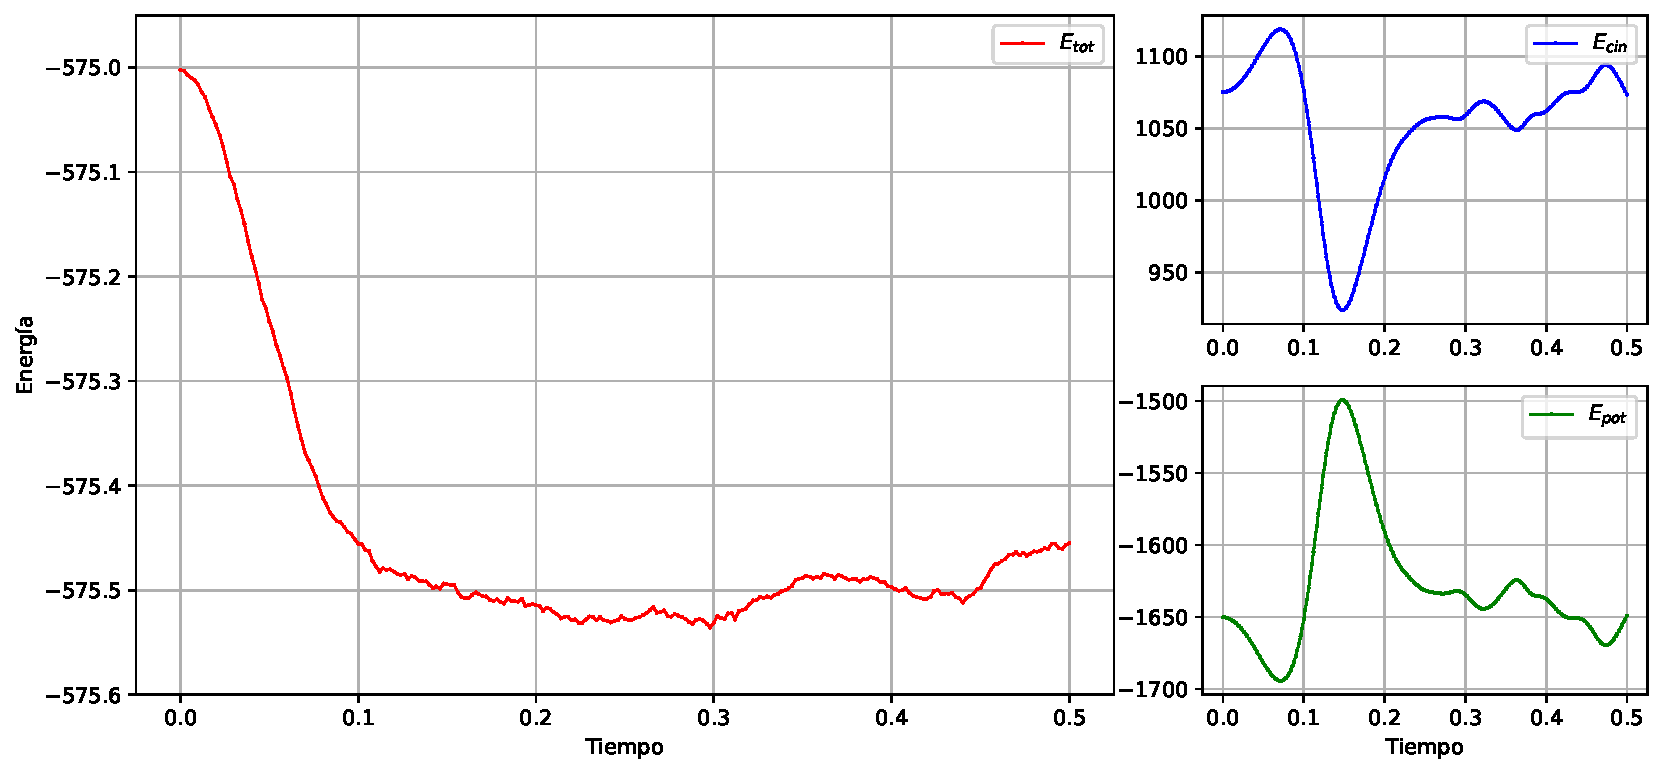
\includegraphics[width=1.0\textwidth]{../../Graficas/Et-equilibra.pdf}
	\caption{evolución de la energía total, cinética y potencial desde la configuración fcc y 5000 pasos.}
	\label{Fig:01}
\end{figure}	


Como podemos ver existe una caída de energía total hacia $-575.5$ sobre la cual, tras los 2000 pasos comienza a oscilar, es decir, se comienza a equilibrar en $-575.5$. La razón por la que sucede esta caída tan repetida es que la configuración inicial es muy simétrica, y por tanto está muy lejos del equilibrio, por lo que su evolución, y los datos que podamos obtener de ella no corresponderá a una colectividad microcanónica de $E=-575$. Entonces lo que tenemos que hacer, para que la simulación tenga la energía deseada, será reescalar las velocidades reescalar las velocidades (adecuándose a la energía cinética que necesitamos para que $E=575$), asegurándonos que el momento total se mantenga cero, al igual que hicimos en el ejercicio anterior (mismo algoritmo mismo proceso).


\begin{figure}[h!] \centering
	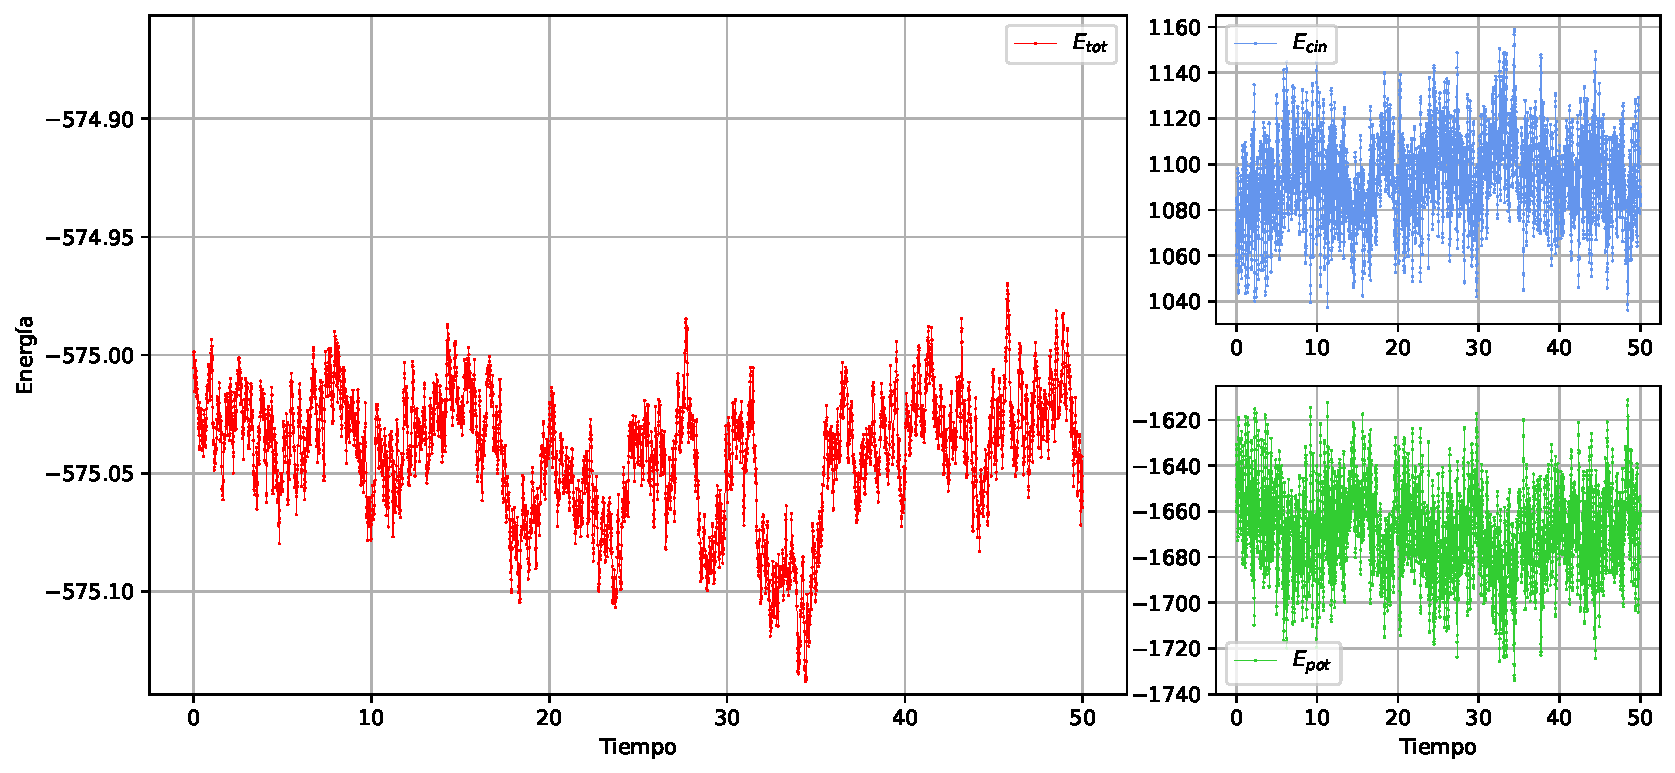
\includegraphics[width=0.9\textwidth]{../../Graficas/Obligatorio2/Et-equilibra-500K-1.pdf}
	\caption{evolución de la energía total, cinética y potencial 500000 pasos.}
	\label{Fig:02}
\end{figure}	

Como podemos ver, a diferencia de la anterior inicialización, en esta no habrá un salto de energía, ya que al haber dejado que ocurrieran 5000 pasos (aunque fuera en otra colectividad microcanónica), la configuración de las partículas ya no es simétrica, y por tanto estará mucho más cerca del equilibrio en la colectividad deseada, por lo que ahora podemos hacer un número mucho más elevado de pasos. Con $\num{5e5}$ serán suficientes. Ahora lo que resta sería usar los datos de las energías cinéticas, potenciales, totales, así como las velocidades de cada una de las 500 partículas en las 3 direcciones (entre otros) para ver si realmente hemos llegado al equilibrio.  

\begin{table}[h!] \centering
	\begin{tabular}{c|c|c}
		& $E_t$ & $s(E_t)$ \\ \hline
		$1^o$ &-575.0422 & 6.9e-09  \\ \hline
		$2^o$ & -575.0044 & 1.0e-08 
	\end{tabular}
	\caption{Valores de las medias para cada interacción e incertidumbre asociada a la media.}
	\label{Tab:01}
\end{table}

Aunque la configuración si se llegue a equilibrar (véase optativo 2), nosotros decidimos realizar una repetición extra, ya que oscilaba sobre un valor de la energía suficientemente alejado de -575 como para tomar la decisión de realizar una vez los 500K pasos, tal y como se puede comprobar en la tabla \ref{Tab:01}. De este modo lo que hacemos es volver a aplicar el algoritmo que nos permite cambiar la energía, y corremos la simulación. Así obtenemos la gráfica \ref{Fig:03}, que oscila más cerca de -575 (vemos que el valor ahora difiere en milésimas y no en centésimas). También se alcanza el equilibrio en esta con mayor celeridad.

\begin{figure}[h!] \centering
	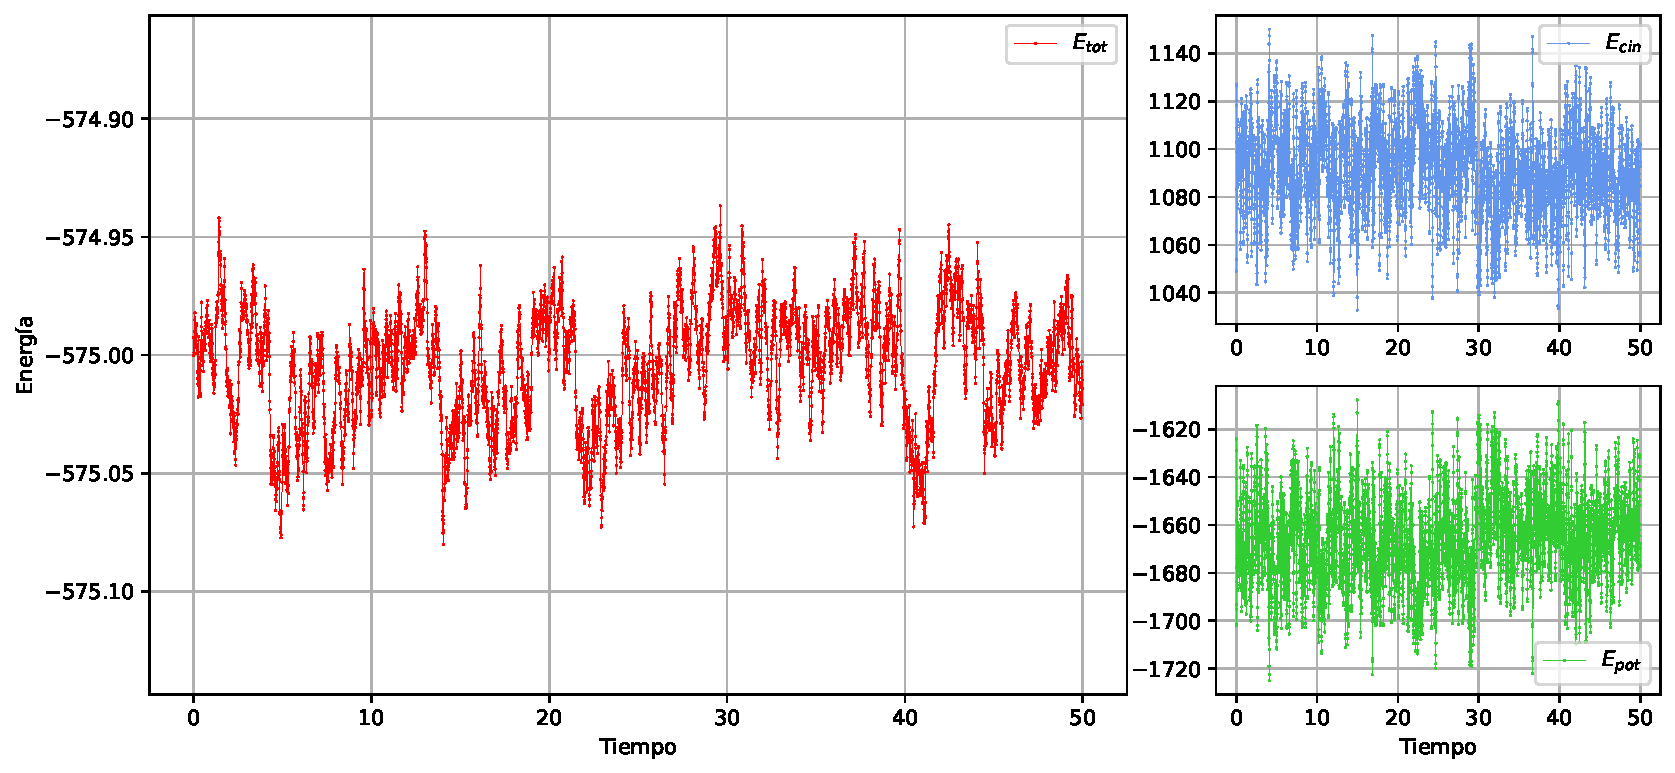
\includegraphics[width=1.0\textwidth]{../../Graficas/Et-equilibra-500K-2.pdf}
	\caption{evolución de la energía total, cinética y potencial 500000 pasos.}
	\label{Fig:03}
\end{figure}	

\subsection{Implementación en Fortran}

Una vez dicho todo esto la implementación en fortran del algoritmo es muy sencilla. Ya hemos hecho un breve resumen de que contiene el programa principal en la sección \ref{Sec:02}, ahora haremos un breve esquema de los pasos que se realizan en dicho programa:

\begin{enumerate}
\item Leemos los datos de una configuración inicial (posiciones, velocidades, aceleraciones, energías).
\item Hacemos un lazo con un número $k$ de pasos. En cada paso avanzaremos un instante $\Delta t$. En este bucle llamaremos en cada interacción a la subrutina Verlet, que nos devolverá la nueva configuración en $t+\Delta t$. Esta a su vez llamará a la subrutina Potlj para calcular los valores de la energía potencial y las aceleraciones (fuerzas). Cada 100 interacciones guardará los datos de las energías y las 3 velocidades de cada una de las 500 partícula que se usarán para el opatativo 1.
\item Una vez acabado el lazo escribirá la nueva configuración en los mismos archivos donde leyó la configuración inicial.
\end{enumerate}

\section{Conclusiones}

Una vez dicho todo esto ya podremos dar por concluido el proceso por el que llegamos a la equilibración, ya que los resultados en principio son satisfactorios, aunque la última palabra sobre si realmente hemos llegado a la equilibración la tendrá el optativo 1 (como veremos se verificarán todas las condiciones).


\bibliography{Bibliografia.bib}
\bibliographystyle{unsrt}
	
\end{document}	
